\chapter{Theoretical Description}
\HtmlMetaDescription{This chapter describes the CFT processor from a
  theoretical perspective.}
%\HtmlMetaGoogleDescription{}
%\HtmlMetaBanner{}
%\HtmlMetaTags{}

This chapter describes the CFT processor from a theoretical
perspective.

For a hardware description of the units described here and more minor ones
beyond the scope of a theoretical discussion, please refer
to~\ccf{chap:processor-hardware-description}. For a description of the
processor's programming model, please refer to~\ccf{chap:programming-model}.

The CFT processor was purposefully designed to be very simple. This
allows it to be built with relatively simple manual techniques, but
also makes it easier to debug, maintain and reason about.

To keep things simple in these days of immense memory, the CFT is a
\gls{von Neumann architecture}: it uses the same memory for both
programs and data, allowing the two to be mixed.

Like many traditional architectures, it is an \abbr{ABA}: operations
usually use a single, main register to hold all values from or to
memory.

Internally, the design (like most hobbyist designs out there) is built
on microcode hosted on Flash RAM, which allows many bugs in the
processor to be solved by reprogramming the memory rather than
rewiring.

\section{Datapath}

Processors are built out of simple, discrete units connected together
by buses and control signals. The CFT is no different. The processor's
datapath, the way data flows from unit to unit, is shown
in~\fcf{fig:datapath}.

%% \begin{figure}
%% 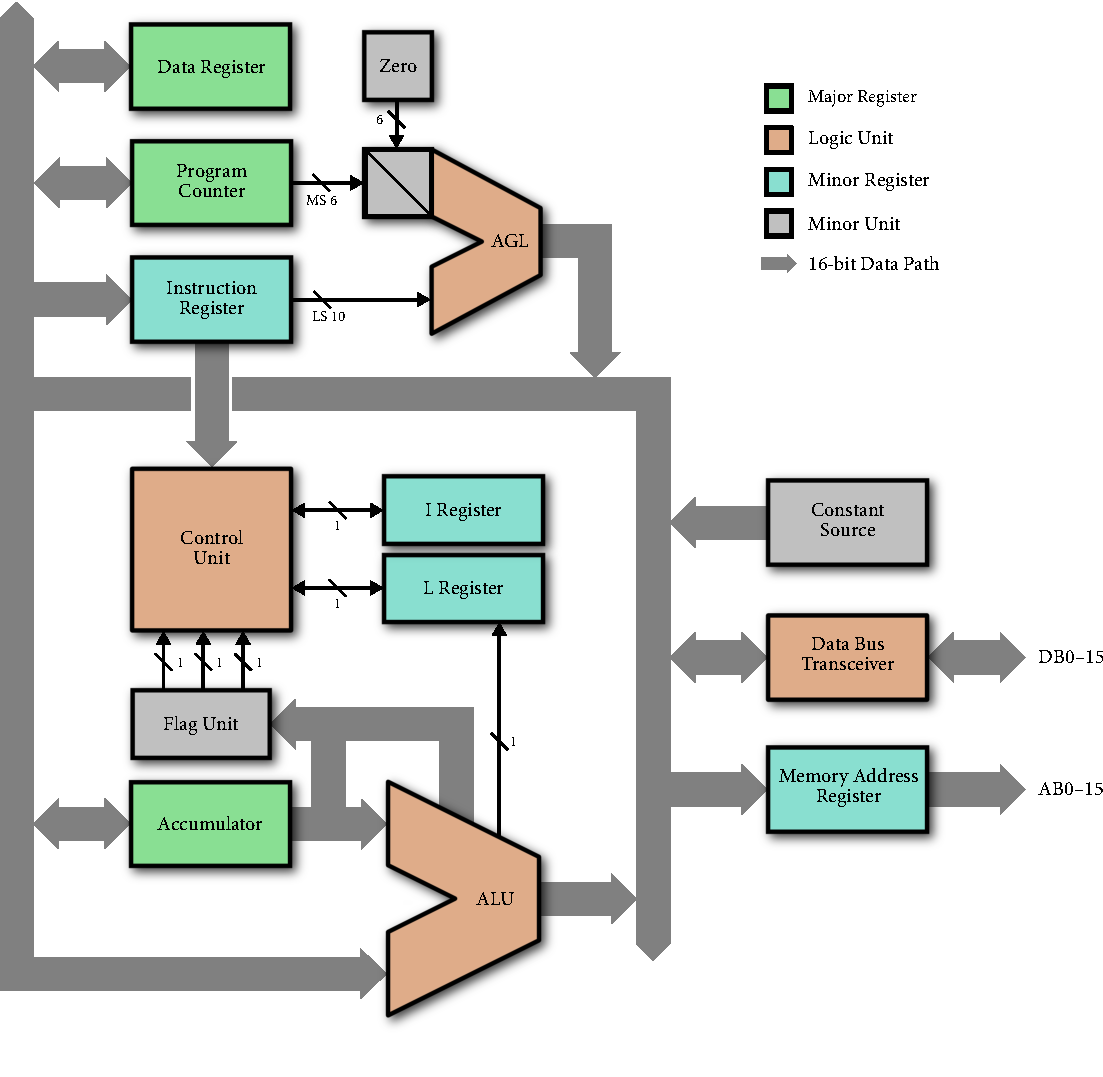
\includegraphics[width=0.95\columnwidth]{figs/datapath2.pdf}\vspace{2em}\\
%% \caption[CFT Datapath]{\label{fig:datapath} The CFT Datapath. }
%% \end{figure}
\begin{figure}
\inputfigure{figure-datapath3}
\caption[CFT Datapath]{\label{fig:datapath} The CFT Datapath. }
\end{figure}

The datapath is organised around a single internal bus (showing surrounding the
datapath diagram), the \IBUS{}. Modern processors use multiple internal buses
or buses segmented into so-called {\em pipelines\/}: this allows one processor
unit to start work before the previous one has completed, increasing processing
speed and complexity of the design. In contrast, the \IBUS{} is not
pipelined. At any given time, at most one unit is writing to it, and (in normal
circumstances) at most one unit is reading from it.

This precludes pipelining techniques, but keeps the processor's behaviour easy
to visualise and implement. A number of units may either write to the \IBUS{},
or read from it. The \IBUS{} may also be connected to the external \DBUS{} via
the Data Bus Transceiver, so that data can be exchanged between the processor
and its peripherals.

The Control Unit (near the top right corner) is not directly attached to the
\IBUS{}, but controls the rest of the processor. To do so, it looks up the
values of various registers and flags on a large table of \gls{microcode} and
activates control signals as dictated by the table, driving the rest of the
processor.
%%  These control signals specify, at any
%% given time and for any given input, which unit (if any) should write to the
%% \IBUS{}, and which unit should read from it. It also controls how flow control
%% (decisions) are made. The Control Unit essentially examines the current state
%% of the machine and derives a new state for it --

The \ALU{} is responsible for arithmetic and logic operations
operations performed by the processor. It can perform a number of
binary and unary operations. All operations involve the
\gls{Accumulator} (AC — see below) as one of the operands. Binary
operations involve the current value of the \gls{Accumulator} and the
value of the \IBUS{}. Unary operations involve only the
\gls{Accumulator}. The \ALU's operations update some of the flags used
by the control Unit.

Ancillary to (and in fact part of) the \ALU{} is the Constant Store,
which can provide a small number of constant values to the
\IBUS{}. These are useful for a number of operations, such as clearing
registers by assigning them the zero constant, or initialising values
of registers when the machine is reset.

There are three {\em major\/} registers in the datapath: the
\gls{Accumulator} (\A), the Data Register (\DR), and the Program
Counter (\PC). Major registers are 16-bits wide. They may be read from
or written to, incremented by one, or decremented by one.

Of these, the \A{} is used as a general-purpose register, permanently and
directly supplying the left operand of the \ALU, and generating flags used by
the Control Unit in decision making.

The \PC{} is used to store the location in memory of the next instruction to be
executed.

The \DR{} is used to temporarily store intermediate addresses used for indirect
memory accesses but may be generally used by the microcode as a scratch
register.

A number of {\em minor registers} are also available. These are either narrower
than 16 bits, or have various restrictions placed on them.

The Interrupt (\Ireg{}) register is a single-bit register that controls whether
asynchronous interrupts (e.g. peripherals needing attention) may temporarily
stop the processor.

The {\em Link Register} (\Lreg) is a versatile single-bit register: it is used
as a flag, a carry out bit, carry in bit, a borrow bit, or a shift register,
and is usually treated as a one-bit extension of the \A{} register.

The Overflow (\Vreg{}) register is a single-bit flag set by the ALU if an
addition has generated a result that will not fit 16 bits. This is used for
signed, two's complement arithmetic: the \Lreg performs the same for unsigned
arithmetic.

The Zero (\Zreg{}) register is set if and only if all the bits of the \AC{} are
zero. It is commonly used for decision making.

The Negative (\Nreg{}) register is set if and only if the most significant bit
of the \AC{} is zero. In signed arithmetic, this signifies the value is
negative, but it may be used to simply test that bit of the accumulator. It is
commonly used in decision making.

The \IR{} is a 16-bit register containing the instruction being executed. From
the point of view of the \IBUS{}, it can only be written to, but its value
directs the Control Unit's behaviour directly.

The memory Address Register (\AR{}) is a write-only 16-bit register that stores
an address. When required, it writes this address onto the \ABUS{} to
facilitate external read/write cycles. This address selects a memory location
or device to access.

Memory addresses used for data are calculating by the \AGL{}, which is
responsible for implementing addressing modes. The \AGL{} can generate 16-bit
addresses either close to the current instruction (by using the top bits of the
\PC{}), or near the beginning of memory (by zeroing the top bits).

The Reset unit is responsible for initialising the state of the processor on
power on or cold reset. It establishes the initial value of the \PC{} and other
registers, and times reset signals sent to peripherals.

Finally, the \unit{MBU} is a recent addition to the processor: it used to be an
external peripheral but has become so useful it was absorbed by the processor
proper. It extends the memory address space of the CFT from 16 bits to 21 bits
by implementing a simple memory banking scheme.

\section{The Control Unit}
\label{sec:control-unit}

The Control Unit is made out of a number of smaller units. In their
entirety, they form a complex state machine or a number of smaller
ones.

\subsection{Major States}
\label{sec:major-states}

The major states of the processor are fairly conventional, as are the transitions between them:

\begin{description}
\li{Reset.} The initial state of the processor. This state is
  entered asynchronously when computer is reset, and remains in this state for
  a set number of clock periods, according to the operation of the reset
  sequencer. During the reset state, slow units stabilise (after being powered
  on, or after a brown out), and numerous registers in the computer are cleared
  to sane values.
  %the \ns{RESET} line is asserted. The processor remains in this state until
  %the reset state machine deasserts \ns{RSTHOLD}, usually after a hardwired
  %number of clock cycles. In the Reset state, internal state is cleared, and
  %the \PC{} is set to the reset vector (\hex{FFF0}).

\li{Fetch.} In this state, the processor performs a memory read to
  get the contents of the \IR, which implicitly jumps to the appropriate
  microprogram, and to the Execute state. The Fetch state is entered at the end
  of the Reset state; at the end of the Stop state once the computer is no
  longer halted; at the end of the Interrupt state once the interrupt
  microprogram has executed; and at the end of the Execute state, when the
  microprogram signals its end — the Fetch-Execute loop forms the implicit Run
  state. In fact, Fetch and Execute are not explicitly signalled: Fetch is
  simply the first memory read cycle of a microprogram, and Execute is the
  remainder. The distinction is only useful in theory\footnote{And on the front
    panel, which actually includes Fetch and Execute lights, decoded based on
    the value of the Control Unit \register{μPC}.}.

\li{Execute.} In this state, the instruction retrieved in the
  Fetch state is executed. This state is only entered at the end of the Fetch
  state and is where all the processing is carried out. At the end of the
  Execute state, the processor usually re-enters the Fetch state to retrieve
  the next instruction, but may also enter the Interrupt state.

\li{Interrupt.} The Interrupt state is entered at the end of the Execute state
if an interrupt has been previously been signalled and interrupts are
unmasked. In this state, the processor saves certain registers and jumps to a
hardwired location holding an interrupt service routine. The actual workings of
interrupts are slightly more complicated than this, as outlined in
\cf{sec:interrupts-state-machine}.
  %sets the \PC{} to the hardwired interrupt vector (\hex{FFF8}).

\li{Stop.} In this state, the processor's microprogram counter
  (\UPC) is inhibited, freezing the processor. The clocks are still
  running, allowing peripherals that use them to operate. This state is entered
  while the computer is halted. The processor's design is fully static, so it
  may stay in the Stopped state indefinitely.

\end{description}

\begin{figure}
  \centering
  \inputfigure{figure-major-states}
  \caption[CFT Processor Major States]{\label{hard:proc:major-states}CFT Processor Major States:
    Reset (R), Fetch (F), Execute (E), Stop (S), and Interrupt (I).}
\end{figure}

\subsection{The Wait State}

The Wait State is a transient, astable state. It may be entered at any time,
though it has special meaning during memory or I/O cycles and is easier to
generate during them. As long as a wait state is signalled, the control unit
protracts its current operation. Wait states are meant to be used with devices
too slow to handle the processor's read or write cycles. They allow most of the
processor to operate at its top speed, slowing down only when communicating
with such devices.


%% The Wait State is a transient state. It may be entered at any time
%% when \ns{WS} is asserted, though it has special meaning during memory
%% or I/O cycles.

%% Once the \ns{WS} signal is deasserted, the processor resumes its
%% previous operation at the next clock tick.

%% \todo{Describe this in detail.}

\subsection{The Fetch-Execute Cycle}
\label{sec:processor-cycle}

The processor spends almost its entire runtime flipping between the
Fetch and Execute states. This is known as Fetch-Execute Cycle and
follows this algorithm:

\begin{enumerate}
\item \IR{} ← mem[\PC]: an instruction is read from the memory address contained in the \PC.
\item \PC{} ← \PC{} + 1: the PC is incremented by one.
\item The instruction is decoded.
\item The instruction is executed.
\item Go to step 1.
\end{enumerate}

These steps are implemented at the microcode level with a level of
parallelism. The first two steps take two clock ticks (known as
clock cycles): memory accesses take two cycles, at the end of
which the \PC{} is incremented. Instruction decoding happens during
this time as well. Instruction execution begins with the third cycle
and can last several cycles.

The fetch-execute cycle of the CFT is implemented in microcode. Almost
every microprogram begins with two microcode instructions to fetch the
next instruction from memory and increment the \PC. The part of each
microprogram up to and including the incrementing of the \PC{} is
conventionally called the fetch state, though the computer treats it
like ordinary microcode processing. In fact, the only point where
Fetch/Execute is displayed is on the front panel for the user's
convenience.

\subsection{The Clock Cycle}

Each clock cycle itself consists of four stages, T1-T4. They are
controlled by the four phases of the main clock. Each phase has a 90°
difference from the previous one, and each lasts 25\% of the nominal
clock period. With the clock running at 4~MHz (250~ns processor
cycle), each phase lasts ¼×250~ns, or 62.5~ns.

\begin{description}
\item{\bfseries T1:} the microprogram counter increments, generating a
  new microprogram address. A microcode memory lookup begins.
\item{\bfseries T2:} the microcode memory lookup concludes. With 70\,ns
  ROMs, the second phase must be used to wait for the signals to
  stabilise. As this happens, the decoding unit (which is
  asynchronous) decodes the micro-instruction vector into read enable
  signals and write strobe enable signals for the various units.
\item{\bfseries T3:} one of various things can happen at this point.
  \begin{itemize}
    \item If no data transfer is required by the micro-instruction, the
      processor goes idle.
    \item If a data transfer between internal processor units is
      needed, the unit to be read from drives the \IBUS{} with its data.
    \item If a memory or I/O read is requested, \ns{MEM} or \ns{IO} is
      asserted as appropriate. \ns{R} is also asserted at this
      time. This instructs the memory or peripheral to select chips
      and initiate a read cycle. During this phase, the memory or
      peripheral may signal a \ns{WS} to temporarily delay the onset
      of the next phase.
    \item If a memory or I/O write is requested, \ns{MEM} or \ns{IO}
      is asserted as appropriate. This instructs the memory or
      peripheral to select chips and initiate a write cycle. Data is
      driven onto the \IBUS{}, and the \DBUS{} is connected to the
      \IBUS{} to provide valid data for the external device. During
      this phase, the device may assert \ns{WS} to temporarily delay
      the onset of the next phase.
  \end{itemize}
\item{\bfseries T4:} one of various things can happen at this point.
  \begin{itemize}
  \item If no data transfer is required by the micro-instruction, the
    processor remains idle.
  \item If a data transfer between internal processor units is
    needed, the appropriate write enable signal is asserted at this
    point, and the unit latches data from the \IBUS. This also
    happens for memory or I/O reads.
  \item If a memory or I/O write is requested, \ns{W} is
      strobed. The external device latches or clocks data
      accordingly.
  \end{itemize}
\end{description}

\begin{figure*}
\centering
\inputfigure{figure-processor-cycle}
\caption[Phases of a processor cycle]{\label{fig:processor-cycle} The
  four phases of a processor cycle. Please note that the microcode
  fetch and decode stages happen asynchronously, since microcode ROM
  access times are higher than 25\% of the clock period. The \DBUS{}
  is never accessed during the first half of the processor cycle,
  which allows other devices (such as a VDU or DRAM refresh circuitry)
  to access the bus.}
\end{figure*}

%% \subsection{Autoindex Logic}

%% If, at the time an instruction is fetched, the \IR{} contains a
%% pattern that matches \bin{XXXX1100'1XXXXXXX}, the internal Autoindex
%% state is entered until the next instruction is fetched. This selects
%% the special indirect indexed addressing modes where locations in
%% memory known as Index Registers are automatically incremented after
%% each use.

\section{The Instruction Register}

This is a simple 16-bit register. It receives its value from the
\IBUS. It never emits its value {\em to\/} the \IBUS. Instead, bits
from it are sent to various other units which act upon them.

The highest five bits (bits 15–11 inclusive) are used to select which microprogram to
run. This sets the instruction and (in most cases) selects either the
direct or indirect addressing mode families.

Bit 10 controls the behaviour of the \AGL to select between the
page-local and page-zero addressing mode families.

Bits 9 to 0 inclusive usually contain the instruction operand but can
be checked individually by the Control Unit to implement special
instructions.

\section{The Major Registers}
\label{sec:major-registers}

The three major registers are the Program Counter (\PC), Data Register
(\DR) and Accumulator (\AC). The \PC{} holds the address of the next
instruction to be executed; the \DR{} is used internally as a
temporary register to implement indirect addressing; and the \AC{} is,
of course, the main register of the machine, fully accessible at the
machine code level.

All three registers are 16-bit wide. Each register may be incremented
or decremented directly and quickly, without involving the \ALU. This
simplifies microcode design significantly and allows for a certain
degree of parallelism.

Since none of these registers are truly general purpose registers,
there are some exceptions: the \PC{} does not need to support
decrementing. The output of the \AC{} is used to generate the
\Zreg{} and \Nreg{} flags. If the \AC{} wraps around during
incrementing or decrementing (carry or borrow), the \Lreg{} is
toggled.

\section{The Arithmetic/Logic Unit}
\label{sec:alu}

The \ALU{} and Constant Store allow the processor to perform
arithmetic and logic operations, and contains useful constants. As is
often the case, this is a very complex unit.


It receives 33 bits of input (the \LAC{} vector and the current
value of the \IBUS), several control signals. The control signals
select an operation to be performed based on the value of the \IR.

Depending on the required operation, the \ALU{} outputs between 16 and
18 bits of data: 16 bits of are placed on the \IBUS. When required,
the remaining bits update the \Lreg{} and \Vreg. Microcode almost
always writes the ALU's result back to the \AC{}.

The operations supported by the \ALU{} are as follows:

\begin{description}

\item{\bfseries Addition:} the value of the \AC{} is added to the
  value on the \IBUS. Carry out from the addition toggles the \Lreg,
  while the \Vreg is updated to indicate signed addition
  overflow. This operation supports both \gls{Twos Complement} signed
  and unsigned addition. With Two's Complement, the same operation may
  be used for subtraction.

\item{\bfseries Bitwise AND:} the value of the \AC{} is conjuncted
  with the value on the \IBUS. Each bit of the result will be set if
  and only if {\em both\/} corresponding bits of the two operands are
  set.

\item{\bfseries Bitwise OR:} the value of the \AC{} is disjuncted with
  the value on the \IBUS. Each bit of the result will be set if and
  only if {\em either\/} of the corresponding bits of the two operands
  are set.

\item{\bfseries Bitwise Exclusive OR:} the value of the \AC{} is
  disjuncted (according to the rules of XOR) with the value on the
  \IBUS. Each bit of the result will be set if the corresponding bits
  of the two operands differ. This operation can test for equality but
  has numerous other applications.

\item{\bfseries Bitwise NOT:} a unary operation. The result contains
  the complement of each bit of \AC{}. Bits in the result are set if
  the corresponding bit in \AC{} is clear and vice versa.

\item{\bfseries Left 1-bit Roll:} a unary operation. The bits of the
  \LAC{} vector are rotated left one place in a circle: the value
  of the \Lreg{} is assigned to bit 0 of the \AC{}; bit 15 of the
  \AC{} goes to \Lreg{}. This is a very useful operation that can be
  used, among other things, to divide a number by two.

\item{\bfseries Right 1-bit Roll:} a unary operation. The bits of the
  \LAC{} vector are rotated right one place. This is a very useful
  operation that can be used, among other things, to multiply a number
  by two.

\item{\bfseries Left 4-bit Roll:} a unary operation. The bits of the
  \LAC{} vector are rotated left four place in a circle. In
  certain cases, this operation may be used to divide a number by
  16.

\item{\bfseries Right 4-bit Roll:} a unary operation. The bits of the
  \LAC{} vector are rotated right four places. In certain cases,
  this operation may be used to multiply a number by 16.

\end{description}

The \ALU{} can also emit the constants \hex{0000}, \hex{0001},
\hex{0002} and \hex{FFF8}. The first three are used to save temporary
copies of the \PC{} during various operations. \hex{FFF8} is the
location in memory of the Interrupt Service Routine.

\section{The Address Generation Logic}

The \AGL{} is responsible for converting 10-bit instruction operands
to 16-bit addresses. To do this, it examines bit 10 in the \IR. If the
bit is set, the top six bits of the address will be zero. If the bit
is clear, the top six bits of the address are taken from the value of
the \PC{} when the instruction fetch started, before incrementing.

This implements two families of addressing modes: page-local and page
zero. In page-local modes, machine code can access data in the same
1,024 word page it is located. In page zero mode, the first 1,024
words are always accessed. The first page is called Page Zero and can
contain globally accessible values. In PDP-8 terminology, these are
called ‘registers’, and bit 10 in the \IR{} is the ‘R’ bit.

\section{The Address Register}

This is a simple 16-bit register that can only be written to using the
current value of the \IBUS. It controls the external Address Bus
during memory and I/O access cycles.

\section{The Data Bus Driver}

The Data Bus driver allows the \IBUS{} to be connected to the external
Data Bus. This, coupled with the Address Bus, allows the computer to
exchange data with memory and I/O devices.

The driver has three states of operation: it can isolate the two buses
from each other; it can allow the \IBUS{} to drive the Data Bus for
write operations; or it can allow the Data Bus to drive the \IBUS{}
for read operations.

\section{Reset Circuitry}

The reset circuitry generates appropriate reset signals as necessary,
and prepares the processor for operation.

To do this, it uses a number of different sources for reset signals
including the front panel and power supply's health status (for
brown-out detection). While a reset signal is held active, the
processor is immediately halted and the reset sequence begins. During
this sequence, the reset circuitry puts the value \hex{FFF0} on the
\IBUS{}, while the processor repeatedly writes this value to the \PC{}
and resets its other registers.

The repetition allows the clock generator and processor to stabilise
during a cold start, but also generates a long reset pulse for any
peripherals connected to the processor. Many peripherals need reset
pulses many microseconds in length, and the reset sequence is
calibrated to fit such peripherals.

At the end of the sequence, the reset signal becomes inactive, and the
Control Unit enters the Fetch-Execute Cycle, starting execution at the
reset address \hex{FFF0}.

\section{The Memory Banking Unit}

The \MBU{} is a full-blown peripheral absorbed by the processor for
its utility. It expands the 16-bit address space of the CFT processor
to 21 bits.

To do this, it divides the 65,536 Word address space into eight 8,192
Word banks, each of which may ‘contain’ 8,192 Words from the a 2 MWord
(21-bit) memory address space. In short, the most significant three
bits of an address are mapped to eight bits: 16-3+8 = 21~bits.

The \MBU{} thus has eight 8-bit registers. Whenever the Address
Register receives an address, the \MBU{} uses the most significant
three bits to select one of the eight registers, and outputs its value
on the 8-bit \AEXT{} bus. Memory cards can the use these eight bits
and the least significant 13 bits of the Address Bus to generate a
physical address.

On reset, the \MBU{} contains a ‘hard mapping’, which can map either
64 KWords of RAM or 32 KWords of RAM and 32 KWords of ROM to the
address space. The selection can be made using a switch on the front
panel.

The ‘soft mapping’ where all eight registers are freely defined may be
activated by configuring the \MBU{} via the processor expansion bus,
like an ordinary peripheral.

The soft/hard status of the \MBU{} is usually shown on the front
panel.


%% \section{Interrupts}

%% \chapter{Hardware Description}
%% \label{chap:processor-hardware-description}


%% The CFT processor is made up of a number of relatively simple units connected
%% in way that causes complex (and in fact, Turing Complete) emergent
%% behaviour. The units are as follows:

%% \begin{description}
%%   \item{\bfseries Clock Generator}. This simple unit generates appropriately
%%     phased clocks from one of three clock sources, and allows stopping the
%%     clock and single-stepping.

%%   \item{\bfseries Reset Sequencer}. Handles reset inputs and performs the reset
%%     sequence.

%%   \item{\bfseries Microcode Sequencer}. The nerve centre of the Control
%%     Unit. Based on a number of inputs and a microcode store, this unit outputs
%%     appropriate control signals to drive the other units in the approproriate
%%     sequence.

%%   \item{\bfseries Unit Decoders}. Decodes microcode sequencer vertical signals
%%     to strobes driving individual units.

%%   \item{\bfseries Skip/Branch Logic}. This unit implements flow control by
%%     signalling the Microcode Sequencer (when it requests this) when a microcode
%%     branch is required. This is also used to perform \gls{machine code}-level
%%     skips.

%%   \item{\bfseries Address Generation Logic}. This unit forms half of the
%%     \glspl{Addressing Mode} of the processor.

%%   \item{\bfseries Instruction Register}. Contains the bit pattern of the
%%     instruction currently being executed. This selects a microprogram for the
%%     Microcode Sequencer to run.

%%   \item{\bfseries Interrupt State Machine}. A state machine that handles
%%     interrupt requests and instructs (when appropriate) the Microcode Sequencer
%%     to jump to the interrupt microprogram.

%%   \item{\bfseries Data Bus Driver and Wait States}. A unit that connects the
%%     processor's internal bus to the external data bus, and also generates write
%%     waveforms. As a bonus, it also handles requested wait states.

%%   \item{\bfseries Address Register}. Is a write-only register that holds the
%%     addresses used to drive the external Address Bus and can drive it as
%%     required.

%%   \item{\bfseries Program Counter}. A major 16-bit register that holds the
%%     address in memory of the next instruction to execute. It supports reading,
%%     writing and increments.

%%   \item{\bfseries Data Register}. A major 16-bit register used to implement
%%     Indirect \glspl{Addressing Mode}. This register supports reading, writing,
%%     increments and decrements.

%%   \item{\bfseries Accumulator}. The single general purpose register of the CFT
%%     architecture. This register supports reading, writing, increments and
%%     decrements, and also calculates the zero and negative flags for the Control
%%     Unit and \gls{ALU}.

%%   \item{\bfseries Autoindex Logic}. This unit helps implement Autoindex mode by
%%     notifying the Microcode Sequencer when the appropriate addresses are used.

%%   \item{\bfseries I/O Device Address Decoder}. To simplify address decoding for
%%     peripherals, this unit decodes the upper eight bits of the I/O address
%%     space and provides appropriate chip select signals on the expansion bus.

%%   \item{\bfseries Link Register}. A complex single-bit register with complex
%%     set, clear and toggle inputs.

%%   \item{\bfseries ALU Operationg Decocder}. Receives signals from the
%%     Control Unit and drives appropriate parts of the \gls{ALU}.

%%   \item{\bfseries ALU Binary B Register}. Implements the right-hand register
%%     for \gls{ALU} binary operations.

%%   \item{\bfseries ALU Binary Y Register}. Implements the output register
%%     for \gls{ALU} binary operations.

%%   \item{\bfseries ALU Binary Table}. Implements the binary operation function
%%     table.

%%   \item{\bfseries ALU Unary Table}. Implements the unary operation function
%%     table.

%%   \item{\bfseries Flag Logic}. Implements the flag registers attached to the
%%     \gls{ALU}.

%%   \item{\bfseries 8 kWord Memory Banking Unit}. A simple banked memory
%%     management unit that allows 21 bits of physical memory to fit the CFT's
%%     16-bit address space.

%% \end{description}

%% \begin{figure*}
%% \includegraphics[width=0.95\textwidth]{figs/Processor-Board-A.png}\vspace{2em}\\
%% \caption[Layout of Processor Board A]{\label{fig:layout-board-a} Layout of Processor Board A.}
%% \end{figure*}
%% \begin{figure*}
%% \includegraphics[width=0.95\textwidth]{figs/Processor-Board-B.png}\vspace{2em}\\
%% \caption[Layout of Processor Board B]{\label{fig:layout-board-b} Layout of Processor Board B.}
%% \end{figure*}
%% \begin{figure*}
%% \includegraphics[width=0.95\textwidth]{figs/Processor-Board-C.png}\vspace{2em}\\
%% \caption[Layout of Processor Board C]{\label{fig:layout-board-c} Layout of Processor Board C.}
%% \end{figure*}

%% This chapter discusses the theory of operation of the actual hardware
%% implementation of the processor. It discusses how the theoretical CFT
%% architecture can be implemented as hardware. It is broken down by
%% processor unit, including the minor ones, and examines each in an
%% isolated fashion.

%% \section{Clock Generator}

%% The original intention is to run the processor at a clock rate of 4~MHz (a
%% clock period of 250~ns). This is output by the clock generator circuitry. There
%% are four clock phases, all at a 50\% duty cycle, each at a 90° phase
%% difference. For each rising clock edge, there is a synchronous, corresponding
%% falling clock edge 90° away, and vice versa. Some of these clock phases are
%% used directly in the processor (or computer) circuitry. Others are combined to
%% create specific timing pulses or strobes.

%% A 4:1 multiplexer selects one of three clock sources: the fast clock
%% (\ps{FASTCLK}, nominally at 16~MHz), a slower demonstration clock named
%% \ps{SLOWCLK} (around 200–250 Hz) and a creeping clock for testing and microcode
%% debugging called \ps{TESTCLK} (around 20–25 Hz). The multiplexer selects among
%% the three clocks with two input signals from the front panel, \ps{FPFAST} and
%% \ps{FPSLOW}. The following function table is implemented:

%% \begin{center}
%%   \zebra
%%   \begin{tabular}{*{4}{>{\textsf\bgroup}c<{\egroup}}l}
%%     %\noalign{\smallskip}\hline\noalign{\smallskip}
%%     %\hline
%%     \ps{FPSLOW} & \ps{FPFAST} & Mux AB & Clock \\
%%     %\noalign{\smallskip}\hline\noalign{\smallskip}
%%     \hline
%%     L & L & \bin{00} & \ps{SLOWCLK} \\
%%     H & L & \bin{10} & \ps{TESTCLK} \\
%%     X & H & \bin{X1} & \ps{FASTCLK} \\
%%     \hline
%%   \end{tabular}
%% \end{center}

%% To provide a sane clock selection when no front panel is connected, \ps{FPFAST}
%% is pulled high and \ps{FPSLOW} is pulled low. This selects the fast clock.

%% \paragraph{Fast Clock}

%% To ensure a stable clock with maximal accuracy, the fast clock was implemented
%% as a single-part, four pin, 16~MHz crystal oscillator. The only additional
%% component to this clock source is a 100~nF bypass capacitor.

%% \paragraph{Slow Clock}

%% There are fewer concerns about the accuracy of the slow clock, and duty cycle
%% is immaterial since clocks are subdivided and only the positive edge is used —
%% as such, only the overall {\em clock period\/} is important. Thus, it was
%% easier and more flexible to implement the slow clock using a 555 timer in its
%% standard astable configuration, as shown in~\fcf{fig:555-astable}.

%% \begin{figure}
%% \centering
%% 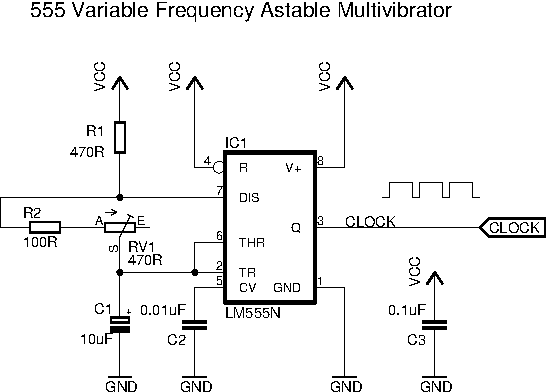
\includegraphics{figs/fig-555-astable.pdf}\\
%% \caption[LM555 in astable configuration] {\label{fig:555-astable}The popular LM555 timer in its astable
%%   configuration, with a variable frequency (and inevitable variable duty
%%   cycle). This one is configured to generate 89–215~Hz frequencies, and is used
%%   as the \ps{SLOWCLK} generator.}
%% \end{figure}

%% \paragraph{Test Clock}

%% The test clock is the same design as the slow clock — in fact, they are both
%% built around the same 556 IC (two 555 timers in one 16-pin \gls{DIP} package).


%%  Each clock source is
%% divided by four internally to generate the four clock phases.

%% \bug{\ps{FPUSTEP} needs to strobe at 2×CLK, this is not very useful.}{} \bug{The slow
%%   clock generators run at ¼ frequency.}{The best way to fix this is to change the 555
%%   capacitor to 2.2µF from 10µF, and adjust the variable resistors.}

%% \todo{Use XOR-based edge detection to generate two pulses (four edges) from one activation
%%   of the \sw{µSTEP} switch.}

%% \todo{Complete this}


%% \begin{figure}
%% \centering
%% \begin{tikztimingtable}
%%   \ns{RAWCLK} & H CL N(A1) 4{CH CL} N(A2) 4{CH CL} N(A3) 4{CH CL} N(A4) 2{CH CL} CH \\
%%   %% \CLOCK{1} (270°)  & L 8H 3{8L 8H} 4L \\
%%   %% \CLOCK{2} (180°)  & 5H 3{8L 8H} 8L \\
%%   %% \CLOCK{3} (90°)   & H 8L 3{8H 8L} 4H \\
%%   %% \CLOCK{4} (0°)    & 5L 3{8H 8L} 8H \\
%%   %% \CLOCK{5}         & L 12H 3{4L 12H} L \\
%%   %% \GUARDPULSE       & 3L ee 3{3H ee 11L ee} 3H ee 8L \\
%%   \CLOCK{1} (0°)       & 3H 3{4L 12H} 4L 6H\\
%%   \CLOCK{2} (90°)      & 7H 3{4L 12H} 4L 2H\\
%%   \CLOCK{3} (180°)     & 11H 3{4L 12H} 2L \\
%%   \CLOCK{4} (270°)     & 3L N(B1) 12H 4L N(B2) 12H 4L N(B3) 12H 4L N(B4) 10H\\
%% %
%%   \extracode
%%   \tablerules
%%   \begin{pgfonlayer}{background}
%%     \foreach \n in {1,...,4}
%%     \draw [help lines] (A\n) -- (B\n);
%%   \end{pgfonlayer}
%% \end{tikztimingtable}
%% \caption{\label{fig:clock-timing} Timing diagram of the four-phase clock generator.}
%% \end{figure}


%% \begin{figure}
%% \centering
%% \begin{tikztimingtable}
%%   \CLOCK{3}    & H CL 4{CH CL} N(A2) 4{CH CL} N(A3) 4{CH CL} N(A4) 2{CH CL} CH \\
%%   \ns{RESET}   & 10H N(A1) 3L ;[dotted] 15L; 7L H ;[dotted] 15H; 10H \\
%%   \ns{RSTHOLD} & 10H 3L ;[dotted] 15L; 8L N(B3) ;[dotted] 15L; 10H \\
%%    \IBUSn{0–15} & 10U{} N(B1) 41D{\hex{FFF0}} N(B4) 10U{} \\
%% %
%%   \extracode
%%   \tablerules
%%   \begin{pgfonlayer}{background}
%%     \foreach \n in {1,4}
%%     \draw [help lines] (A\n) -- (B\n);
%%   \end{pgfonlayer}
%% \end{tikztimingtable}
%% \caption[Reset waveform]{\label{fig:reset-timing} Reset waveform. The width of \ns{RSTHOLD} has
%%   a guaranteed, configurable minimum width and its rising edge is synchronous
%%   to the rising edge of \CLOCK{3}.}
%% \end{figure}


%% \section{Reset Logic}

%% The Reset Logic is a simple 8-bit counter, clocked from the processor clock to
%% ensure the reset pulse is synchronised with the processor sequencer.

%% A number of open drain reset inputs are combined together and fed into the
%% counter's active low reset pin. These include:

%% \begin{itemize}
%% \item The front panel \ns{FPRESET} input. This is connected to a toggle switch
%%   and allows the user to reset the computer manually.
%% \item The power supply \ps{POWEROK} signal. The power supply asserts this when
%%   the power output is healthy. The signal is clear when the power supply is
%%   still stabilising after initial power up, or when a brown-out is
%%   detected. Interpreting it as the imaginary active-low ‘\ns{POWERBAD}’ signal
%%   allows us to reset the machine on brown-outs {\em and\/} to allow for a
%%   power-on reset sequence.
%% \item When the optional reset button on the reset logic board is pressed.
%% \item When the open drain \ns{RESET} signal is asserted. This allows any number
%%   of external drivers of this signal.
%% \end{itemize}

%% When the reset signal goes low, the counter resets and starts counting. A bank
%% of jumpers connects one of the counter's binary outputs to the \ns{RSTHOLD}
%% signal. With the count reset, \ns{RSTHOLD} goes low. When the count progresses
%% enough for the selected bit to go high, \ns{RSTHOLD} goes high
%% (deasserted). This also disables the counter. At this point, the \ns{RSTHOLD}
%% pulse is complete.

%% By selecting which count bit drives \ns{RSTHOLD}, the pulse width can be controlled. In
%% theory, pulse widths of $2^n$ clock periods ($1\leq n\leq 8$) can be used. In practice,
%% because the counter is registered, and the register and count inputs are wired together,
%% the \ns{RSTHOLD} pulse lasts for one extra clock period. Also, since the reset pulse
%% arrives asynchronously, the \ns{RSTHOLD} may be up to one clock period longer yet.

%% With a clock of 4~MHz, the longest reset pulse is 64.25~ms which is fine for most uses:
%% the processor itself is very quick to reset, needing less than one clock period. Other
%% hardware, however, is not as fast. Since a reset sequence also happens when the computer
%% powers up or a brown-out is detected, an extended \ns{RSTHOLD} pulse makes the processor
%% wait for power rail and clock stabilisation (among other potential pitfalls).

%% While \ns{RSTHOLD} is active, the value \hex{FFF0} is driven onto the \IBUS{}
%% using a pair of 74x541 buffers. This is the Reset Vector. The processor uses
%% this value to reset the \PC{} to its initial value.








%% \section{Skip Logic}

%% \lipsum[3-5]

%% \section{Address Generation Logic}

%% The \gls{AGL} is a relatively simple unit, but it provides half of the CFT's
%% addressing modes.

%% The purpose of the AGL is to take the 10-bit operand field of the \IR{} and use
%% it to produce a full, 16-bit address. The source of the most significant six
%% bits depends on the value of the \asm{R} (register) field of the \IR.

%% \begin{description}
%% \li{If \asm{R} is zero}, the upper six bits come from the \PC, so
%%   the address is generated relative to the currently executing
%%   instruction.\footnote{The \PC{} normally holds the address of the {\em
%%       next\/} instruction to be executed, but a special case is needed here,
%%     discussed below.}
%% \li{If \asm{R} is one}, the upper six bits are zero
%%   (\bin{000000}). This allows for addresses in the first 10 bits of memory,
%%   i.e. addresses \hex{0000}–\hex{03FF}.
%% \end{description}

%% In essence, the \gls{AGL} is a 2:1 multiplexer, which, depending on the value
%% of \IRn{10}, outputs either \bin{pppp:ppnn:nnnn:nnnn} (When \IRn{10}$ = 0$,
%% $\mbox{\textsf{page}} × 2^{10} + \mbox{\textsf{offset}}$, where \textsf{page} comes
%% from the \PC), or \bin{0000:00nn:nnnn:nnnn} (When \IRn{10}$ = 1$, \gls{Page Zero}
%% addresses).

%% This is implemented using two \HC{541} 8-bit buffers and an \HC{374} 8-bit
%% edge-triggered latch.

%% The latch receives \PCn{10–15}. It latches this value at the rising edge of
%% \ns{END}, which comes at the very end of an instruction. At this point in the
%% processor's timeline, the PC holds the address of the instruction about to be
%% fetched. As a result, the latch will hold the upper six bits of \PC{} just
%% before instruction fetch, and before it's incremented. The reasoning behind
%% this becomes evident if the case \PC$=$\bin{AAAA:AA11:1111:1111} is
%% considered. When the instruction is fetched, the PC is loading from page
%% {AAAA:AAxx:xxxx:xxxx}. However, at the end of the fetch cycle, the \PC{} is
%% incremented. This wraps around to page $A+1$, and any address generated at that
%% point will access memory from the wrong page. This is an insidious issue
%% because it only appears if an instruction uses local addressing at the very end
%% of a page. It would be unreasonable to expect the programmer to resolve this
%% issue in software, so the latch ensures the instruction set behaves
%% consistently.

%% The output of the latch is controlled by \IRn{10}. When it is low, the latch
%% drives its output pins. When it is high, the output pins are tri-stated. The
%% lines are pulled-down, so they revert to a weak low level, which is equivalent
%% to a page of \bin{0000:00xx:xxxx:xxxx}.

%% These lines drive the upper six inputs of the \gls{MSB} buffer. The remaining
%% two inputs and all eight inputs of the \gls{LSB} buffer are driven by the
%% \IRn{0–9}, which provide the offset within the page.

%% The buffers' outputs remain tri-stated unless the \ns{RAGL} active-low signal
%% is asserted by the Control Unit. When that happens, the buffers drive \IBUS{}
%% with the generated address.

%% To allow future expansion, a six-pin header connected to the
%% pulled-down lines can be used to provide a different page number
%% rather than page zero.

%% \section{The Address Register and Address Bus Driver}

%% The Address Register (\AR) is a minor, 16-bit write-only register. The register
%% is implemented as a pair of \HC{273} 8-bit flip-flops. The flip-flops latch
%% their value on the rising edge of \ns{WAR}. The \AR{} is cleared when
%% \ns{RESET} is asserted.

%% The outputs of the flip-flops, which cannot be tri-stated, are fed into a pair
%% of \HC{541} buffers. The buffers form the \ABUS{} driver. They allow the \AR{} to
%% be tri-stated using the \ns{ABEN} signal (Address Bus Enable). This signal is
%% generated from \ns{MEM} and \ns{IO} by an AND gate according to the following
%% table:

%% \begin{center}
%%   \zebra
%%   \begin{tabular}{*{3}{>{\textsf\bgroup}c<{\egroup}}l}
%%     %\noalign{\smallskip}\hline\noalign{\smallskip}
%%     %\\\hline
%%     \ns{MEM} & \ns{IO} & \ns{ABEN} & Function \\
%%     %\noalign{\smallskip}\hline\noalign{\smallskip}
%%     \hline
%%     H & H & H & \ABUS{} tri-stated \\
%%     L & X & L & \AR{} drives \ABUS{} \\
%%     X & L & L & \AR{} drives \ABUS{} \\
%%     \hline
%%   \end{tabular}
%% \end{center}

%% Thus, the \AR{} drives the \ABUS{} when and only when a memory or I/O cycle is
%% in progress.


%% \section{Autoindex Logic}
%% \label{sec:ail}

%% The Autoindex Logic is a small unit that detects when an address in the range
%% \hex{0080}–\hex{00FF} is referenced. This is done by comparing the Address
%% Register (\AR) against the value \bin{0000:0000:1xxx:xxxx}. The comparison is
%% performed with a \HC{688} 8-bit comparator, using all eight bits plus the
%% active-low cascade input (\ns{G}).

%% The comparator outputs an active low equality signal, \ns{P=Q}, which asserts
%% the asynchronous set signal of half a \HC{74} D flip-flop. The complementary
%% (\ns{Q}) output of the flip-flop is fed into the Microcode Unit, where it is
%% checked and acted upon by whatever microprograms need it.

%% The flip-flop is asynchronously cleared by the \ns{END} signal to reset
%% \ns{AINDEX} at the end of the current instruction. The flip-flop's synchronous
%% functions are not used. Resetting to a known state is also done
%% programmatically — the short reset microprogram asserts \ns{END}, which clears
%% the flip-flop.

%% \ns{AINDEX} is latched for the duration of the instruction because of indirect
%% addressing modes which modify the value of the \AR{} and can potentially
%% de-assert \ns{AINDEX} mid-instruction.

%% \section{The Data Bus Driver}

%% The \DBUS{} driver is a surprisingly complex logic unit responsible for:

%% \begin{itemize}
%% \item Connecting the \IBUS{} to the \DBUS{} when necessary and observing the
%%   proper transfer direction.
%% \item Extending read/write cycles by the appropriate length of time when a wait
%%   state has been requested are active.
%% \item Generating write strobes (\ns{W}) from write-enable (\ns{WEN}) signals as
%%   required.
%% \end{itemize}

%% \subsection{Driving the Buses}

%% The buses are connected when the \ns{BUSEN} signal is asserted. This is
%% generated according to the following table, of which the \ns{WAITING} signal is
%% derived according to~\cf{sec:dbus-driver-waiting}:

%% \begin{center}
%%   \zebra
%%   \begin{tabular}{*{5}{>{\textsf\bgroup}c<{\egroup}}l}
%%     %\noalign{\smallskip}\hline\noalign{\smallskip}
%%     %\hline
%%     \ns{MEM} & \ns{IO} & \ns{T34} & \ns{WAITING} & \ns{BUSEN} & Notes \\
%%     %\noalign{\smallskip}\hline\noalign{\smallskip}
%%     \hline
%%     H & H & X & H & H & Bus idle \\
%%     H & H & H & X & H & Bus idle \\
%%     L & X & X & X & L & Memory cycle in progress \\
%%     X & L & X & X & L & I/O cycle in progress \\
%%     X & X & L & L & L & Wait state \\
%%     \hline
%%   \end{tabular}
%% \end{center}

%% The centrepiece of the driver is a pair of \HC{245} bidirectional
%% transceivers. Their ‘A’ ports are connected to the \IBUS{}; their ‘B’ ports are
%% connected to the \DBUS.

%% The direction pin is connected to \ns{R}, so that the following function table
%% is implemented:

%% \begin{center}
%%   \zebra
%%   \begin{tabular}{*{2}{>{\textsf\bgroup}c<{\egroup}}l}
%%     %\noalign{\smallskip}\hline\noalign{\smallskip}
%%     %\\\hline
%%     \ns{BUSEN} & \ns{R} & Function \\
%%     %\noalign{\smallskip}\hline\noalign{\smallskip}
%%     \hline
%%     H & X & \DBUS{} tri-stated \\
%%     L & H & \DBUS{} drives \IBUS{} (read cycle) \\
%%     H & L & \IBUS{} drives \DBUS{} (write cycle) \\
%%     \hline
%%   \end{tabular}
%% \end{center}


%% \begin{figure*}
%% \centering
%% \begin{tikztimingtable}
%%   Stage            & D{} 5{3D{T1} 3D{T2} 3D{T3} 3D{T4}} D{} \\
%%   \CLOCK{2}        & H N(A1) 3H 3L 6H N(A2) 3H 3L 6H N(A3) 3H 3L 6H N(A4) 3H 3L 6H N(A5) 3H 3L 6H H \\
%%   \ns{T34}         & H 5{6H 6L} H \\
%%   \ns{RESET}       & 2H 3L 57H \\
%%   \ns{MEM}         & 6H 7L 6H 18L 25H \\
%%   \ns{R}           & 7H 5L 8H 16L 26H \\
%%   \ns{WS}          & 20Z 9L 21Z 2L 10Z  \\
%% %
%%   \ns{WAITING}     & 2U 18H 11L 31H \\
%% %% \extracode
%% %%  \tablerules
%% %%  \begin{pgfonlayer}{background}
%% %%    \foreach \n in {1,...,11}
%% %%      \draw [help lines] (A\n) -- (B\n);
%% %%  \end{pgfonlayer}
%% \end{tikztimingtable}
%% \caption[Wait State Waveform]{\label{fig:wait-state} Wait state waveform. The
%%   second pulse of \ns{WS} has no effect because \ns{T34} is high, and because
%%   it does not cross the T4-T1 boundary.}
%% \end{figure*}

%% \subsection{Extending Read/Write Cycles on Wait States}
%% \label{sec:dbus-driver-waiting}

%% The bus protocol for using wait states to extend bus transactions is described
%% fully in~\cf{sec:bus-ws}. In short, when a slow peripheral on the bus is
%% addressed, it may assert the \ns{WS} signal immediately to extend the read or
%% write operation. For write cycles, \ns{WS} must be asserted before the \ns{W}
%% is strobed, which gives a window of approximately 180~ns. Once \ns{WS} is
%% asserted, it must be held low until the rising edge of \CLOCK{1} and must be
%% de-asserted before the rising edge of \CLOCK{2}. If a \ns{WS} strobe occurs
%% entirely outside the T3 or T4 cycle phase, it is ignored.

%% \ns{WS} must be driven by an open-drain gate to allow sharing the line among
%% all peripherals. The \ns{WS} performs two tasks: as described in~\cf{sec:upc},
%% it stops the µPC from counting to the next microinstruction; and it extends the
%% bus transaction by keeping the \IBUS{} and \DBUS{} connected. The latter is
%% performed here by the \ns{WAITING} signal. The waveform is shown
%% in~\fcf{fig:wait-state}.

%% \ns{WAITING} is the complementary output of a \HC{74} D flip-flop. The flip-flop
%% is asynchronously set when the disjunction \ns{T34}$\cdot$\ns{WS} is low (this
%% is generated by an OR gate, which works as a negative logic AND gate by
%% DeMorgan's law). Thus, it is set when a wait state is reuquested during the T3
%% ot T4 cycle phase. The flip-flop's \ps{D} input is pulled low, and it is
%% clocked by the rising edge of \CLOCK{2}. In essence, unless a wait state is
%% still being requested, the rising edge of \CLOCK{2} (i.e. the onset of the T3
%% phase) will clear it. This will allow the bus cycle to complete after the end
%% of the wait state. The flip-flop is also reset asynchronously on \ns{RESET}.

%% \ps{WAITING} (the complement of \ns{WAITING}) is obtained from the flip-flop's
%% \ps{Q} output and is used to inhibit \ns{W} strobes during wait states.

%% %% \question{Why use \ns{WAITING} to extend the bus transaction, when the
%% %%   Microcode Store is stopped and control signals do not change?}{Peripherals
%% %%   generate their \ns{WS} signals when they are addressed, and often {\em
%% %%     while\/} they are addressed. Keeping the bus connected is very }



%% \subsection{Generating Write Strobes}
%% \label{sec:w-strobe}

%% \begin{figure*}
%% \centering
%% \begin{tikztimingtable}
%%   \CLOCK{4}          & 5{6H 2L} 5H \\
%%   \ps{WAITING}       & 20L       14H 11L \\
%%   \ns{MEM}           & 3H 6L 10H 22L 4H \\
%%   \ns{WEN}           & 3H 6L 10H 22L 4H \\
%%   \ns{W}             & 6.5H 1.5L 30.5H 1.5L 5H \\
%% %% \extracode
%% %%  \tablerules
%% %%  \begin{pgfonlayer}{background}
%% %%    \foreach \n in {1,...,11}
%% %%      \draw [help lines] (A\n) -- (B\n);
%% %%  \end{pgfonlayer}
%% \end{tikztimingtable}
%% \caption[Write Strobe Generation]{\label{fig:write-strobe-generation} Write
%%   Strobe generation. This diagram shows two write transactions. The first one,
%%   on the left, is an ordinary write. The second one, centre to right, is one
%%   with a wait state. The asserted \ps{WAITING} signal inhibits the \ns{W}
%%   strobe for two clock cycles. The transaction continues until after
%%   \ps{WAITING} is cleared, to the end of the memory write cycle. }
%% \end{figure*}

%% Most peripherals, including memory, require some time after they are selected,
%% for address decoding to settle, buses to be fully driven, et cetera. They also
%% require these signals to be held after a write pulse. This does not allow the
%% write pulse to start at the same time as the bus cycle starts, nor to end at
%% the same time as the cycle ends.

%% Thus, although the Control Unit directly controls the \ns{R} signal on the bus,
%% it only indirectly controls the \ns{W} signal. Instead, it asserts a \ns{WEN}
%% (Write ENable) signal, and this part of the \DBUS{} driver generates the \ns{W}
%% strobe from it.

%% The \ns{W} strobe is generated by the complementary output of half of a \HC{74}
%% flip-flop. The \ns{D} input is pulled high. When the \ns{CLK} line rises, the
%% flip-flop is set, \ns{Q} is cleared, and a write strobe begins. The strobe is
%% cleared using the asynchrnous reset signal of the flip-flop, when either
%% \ns{RESET} is asserted, or approximately 25–30~ns after \ns{Q} goes low. A
%% feedback from \ns{Q}, delayed by propagation through four gates, is used to
%% clear the flip-flop again.

%% Since bus transactions last until the next microinstruction is fetched from the
%% microcode store, the rising edge of the \ns{W} strobe occurs approximately
%% 15~ns (the $t_{\mbox{\scriptsize PHL}}$ or $t_{\mbox{\scriptsize PLH}}$ delays
%% of the µPC's \HC{161}) plus 50–70~ns (the access time of the microcode store)
%% before the end of the read/write cycle. This gives an address, data and chip
%% select hold time of 65–85~ns, more than enough for most devices.\footnote{Many,
%%   in fact, need {\em no\/} hold time.}

%% Thus, the \ns{W} strobe is asserted on the rising edge of the flip-flop's
%% \ns{CLK} according to the following table and as shown in~\fcf{fig:w-strobe}.

%% \begin{center}
%%   \zebra
%%   \begin{tabular}{*{4}{>{\textsf\bgroup}c<{\egroup}}l}
%%     %\noalign{\smallskip}\hline\noalign{\smallskip}
%%     %\\\hline
%%     \CLOCK{4} & \ns{WEN} & \ps{WAITING} & FF \ps{CLK} \\
%%     %\noalign{\smallskip}\hline\noalign{\smallskip}
%%     \hline
%%     H & X & X &   L \\
%%     X & H & X &   L \\
%%     X & X & H &   L \\
%%     L & L & L &   H \\
%%     \hline
%%   \end{tabular}
%% \end{center}


\section{Interrupt State Machine}
\label{sec:interrupts-state-machine}

Interrupts allow the normal flow of computation to be temporarily stopped in
order to process out-of-order events like user input, or slow devices
completing previously initiated transactions. They are crucial to building a
computer with practical uses, but can be tricky to implement due to their
asynchronous nature. Race conditions and metastability can cause trouble.

The CFT interrupt subsystem is a five-state Finite State Machine. On reset, the
processor starts with interrupts masked, and will ignore any interrupt
requests. Interrupts may be enabled at any time using the \asm{SEI}
instruction. Once enabled, on receipt of an interrupt, the processor completes
the currently running instruction, then executes the Interrupt
Microprogram. The microprogram disables further interrupts, saves the current
value of the \PC~and jumps to the location of the \abbr{ISR}. The ISR
handles the interrupt and usually enables further interrupt requests just
before exiting.

Since the CFT lacks a hardware stack, nested interrupts are not an option. So,
enabling interrupts and exiting the ISR must happen atomically. Otherwise, an
incoming interrupt may jump back to the ISR immediately after the \asm{SEI}
instruction and before the ISR returns. To avoid this, \asm{SEI} waits until
the next \PC-changing instruction (loading, not incrementing) before
enabling interrupts.

The interrupt state machine has five states, as shown
in~\fcf{hard:proc:interrupt-fsm}:

\begin{figure}
  \centering
  \inputfigure{figure-interrupt-fsm}
  \caption[CFT Processor Interrupt State Machine]{\label{hard:proc:interrupt-fsm}Interrupt state transition diagram.}
\end{figure}

\begin{enumerate}

\item {\bf Interrupts Disabled}. This is the initial state on reset. In this
  state, interrupts are ignored. When the \asm{SEI} instruction runs, it
  strobes the \ns{STI} signal. The rising edge of \ns{STI} arms the interrupt
  enable.

\item {\bf Interrupt Enable armed}. Interrupts are still masked in this
  state. When the \PC~is next written to using an \asm{JMP}, \asm{JSR},
  \asm{RET}, \asm{RTI} or \asm{RTT} instruction (or macros involving one of
  them), and on the rising edge of the \ns{WPC} strobe, interrupts become
  fully enabled.

\item {\bf Interrupts Enabled}. In this state, interrupts will be received by
  the processor. If a low level is seen on the \ns{IRQ} line, the state machine
  moves to the Interrupt Armed state. If a \asm{CLI} instruction is executed, a
  low level of the \ns{CLI} signal will reset the state to ‘Interrupts
  Disabled’ and subsequent interrupts will be ignored.

\item {\bf Interrupt Armed}. The state machine remains in this state until the
  currently executing instruction is finished. This is signalled by the rising
  edge of \ns{END} from the Control Unit, at which point \ns{IRQS} goes low to
  acknowledge the interrupt, the Control Unit executes the Interrupt
  Microprogram, and the state machine moves to the next state.

\item {\bf Interrupt Microprogram}. The state machine remains here while the
  interrupt microprogram is being sequenced. During this sequence, interrupts
  will be disabled via a strobe of \ns{CLI}. This resets the state machine to
  the {\em Interrupts Disabled\/} state, and the process cycles.

\end{enumerate}

\begin{figure}
  \centering
  \inputfigure{figure-interrupt-waveforms}
  \caption[CFT Processor Interrupt
    Waveforms]{\label{hard:proc:interrupt-waveforms}Interrupt waveforms. 1.~The
    \asm{SEI} instruction strobes \ns{STI} preparing to enable
    interrupts. \ps{STI-ARMED} is asserted. 2.~When next the \PC~is loaded with
    a value, interrupts are enabled. The rising edge of \ns{WPC} strobes
    \ns{STI-DELAY} disarming the interrupt enable and asserting the \ns{FINT}
    flag to allow interrupts. 3.~With \ns{FINT} low, an incoming \ns{IRQ}
    signals an interrupt request. \ps{FIRQ} goes high to arm the
    interrupt. 4.~At the end of the current microprogram (rising edge of
    \ns{END}), \ns{IRQS} is asserted, both acknowledging the interrupt and
    making the Control Unit execute the Interrupt microprogram. 5.~During the
    microprogram, \ns{CLI} is asserted. Interrupts are disabled and cleared
    (\ps{FIRQ} goes low). 6.~At the end of the microprogram, the state machine
    cycles back to masked interrupts. Control is now in the~\abbr{ISR}.}
\end{figure}



\chapter{Hardware Description}
\HtmlMetaDescription{This chapter describes the CFT processor's
  hardware implementation, in detail.}

This chapter describes the CFT processor's hardware implementation at
the digital electronics level. Most of the units from the theoretical
description feature here, as well as a number of sub-units and units
not worth mentioning in the theoretical description.

\section{Overview}

The CFT Processor is built on four printed circuit boards, designated
PB0 to PB3:

\begin{description}

\item{\bfseries Processor Board 0 (PB0):} contains the Microprogram
  Counter, the Microcode Store, Read/Write Unit Decoders, Address and
  Data Bus signal conditioning, and the optional \abbr{µCB}.

\item{\bfseries Processor Board 1 (PB1):} a complex board that hosts
  the clock generator, reset circuitry, \abbr{SBU}, \abbr{AGL}, the
  \IR{}, the Interrupt State Machine, the Data Bus Driver, the Wait
  State logic, the Write Strobe generator, and \IBUS{} signal
  conditioning and termination,

\item{\bfseries Processor Board 2 (PB2):} hosts the three major
  registers, their front panel buffers, the Address Register (and its
  own buffers), as well as the \Zreg, \Nreg{} flags and the Autoindex
  Logic.

\item{\bfseries Processor Board 3 (PB2):} hosts the \Lreg register,
  the \ALU{} and the \MBU.

\end{description}

\section{Processor Board 0}
\subsection{Microprogram Counter}
\label{sec:upc}

The Microprogram Counter (µPC) is a simple 4-bit counter with reset and dual
count enables. A \HC{161} counter was selected for this. The '161 counts on the
positive edge of \CLOCK{4}, while the count enables are high. These are driven
by \ns{WS} and \ns{HALT}, both pulled up in case the two input signals are
physically unconnected.

The counter resets to zero when \ns{RSTHOLD} is asserted.

The \ns{END} signal and its open drain, external counterpart \ns{ENDEXT} are
ANDed together and fed to the '161's active low load signal (\ns{LD}). This
loads the counter from the \ps{P1}–\ps{P4} inputs, which are permanently tied
to GND. This provides a second reset circuit, when the currently executing
microprogram is finished.

The counter's output provides the four least significant bits of the microcode
address vector, the others being provided by other processor states.

In terms of CFT processor signals, the counter implements the following function table:

\begin{center}
  \zebra
  \begin{tabular}{*{6}{>{\textsf\bgroup}c<{\egroup}}l}
    %\noalign{\smallskip}\hline\noalign{\smallskip}
    %\\\hline
    \ps{CLOCK4} & \ns{RSTHOLD} & \ns{END} & \ns{ENDEXT} & \ns{WS} & \ns{HALT} & Function \\
    %\noalign{\smallskip}\hline\noalign{\smallskip}
    \hline
    X   & L & X & X & X & X & Reset counter to 0 asynchronously.\\
    \tU & H & L & X & X & X & Reset counter to 0.\\
    \tU & H & X & L & X & X & Reset counter to 0.\\
    \tU & H & X & X & L & X & Inhibit counting.\\
    \tU & H & X & X & X & L & Inhibit counting.\\
    \tU & H & H & H & H & H & Increment count (mod 16).\\
    \hline
  \end{tabular}
\end{center}

\begin{figure*}
  \centering
  \inputfigure{figure-microcode-counter}
  \caption[Microprogram Counter Waveforms]{\label{fig:upc-timing} Timing
    diagram of the operation of the microprogram counter (\UPC). The
    counter resets synchronously while \ns{RSTHOLD} is asserted. The
    rising edge of \CLOCK{4} clears it if either \ns{END} or \ns{ENDEXT}
    are asserted, and counting is inhibited when \ns{WS} or \ns{HALT}
    are asserted.}
\end{figure*}


\subsection{Microcode Store}
\label{sec:microcode-store}

\begin{figure}[tb]
  \centering
  \inputfigure{figure-microcode-store}

  \caption[Microcode address vector]{\label{fig:ucode-addr-vector}Microcode
    Address Vector (top) and output control signals (bottom). The Address
    Vector forms the 15–19 bit address (the \ps{μCB} field is optional) for
    three ROMs, each of which outputs 8 bits of the 24-bit wide control
    vector. The control vector, in turn, drives the processor. }
\end{figure}

The microcode store is the heart of the Control Unit. It consists of a large
truth table mapping 15 or 19 (if the \abbr{µCB} extension is installed) bits of
input to 24 bits of output. The input depends on the current instruction being
executed and other state bits of the processor.

From the electronics perspective, the microcode store is implemented as three 4
MBit (524,288×8 bits each) Flash devices. The devices are reprogrammable, which
allows the microcode to be corrected and updated, although they have to be
removed from their sockets for this to be done.

All three ROMs receive the same address vector. Each outputs 8 bits of the
control vector in parallel. To minimise access times, the chips are permanently
selected by tying their \ns{CE} pins to ground. Since in-circuit programming is
not not available, the \ns{WE} pins are tied to Vcc, turning the Flash devices
into ROMs.

The output enable pins (\ns{OE}) are low, except when \ns{HALT} or \ns{RESET}
are asserted. With the processor halted (or in the early stages of resetting),
the ROMs are in a high impedance state, allowing other units (such as the front
panel controller) to control the processor's units. Pull-up and pull-down
resistors weakly tie the control signals to safe (idle) levels.


\section{Microcode Format and the Control Unit}
\label{sec:microcode-format}

A full discussion of the microcode architecture from a software point of
view can be found in~\ccf{chap:microcode}.

Microcode is a multivariate function that accepts a number of inputs, the
address vector, and outputs a number of control signals. 

The address vector is made up of the following fields, in order of increasing
bit significance:

\begin{description}
\item \textbf{Bits 0–3: \UPC}. This is the output of the microcode counter as
  described in~\cf{sec:upc} and represents the offset inside a
  microprogram. The remainder of the bits identify different microprograms.
\item \textbf{Bit 4: \ns{AINDEX}}. Asserted by the Autoindex Logic when autoindex memory locations are accessed. The Autoindex Logic is described in~\cf{sec:ail}.
\item \textbf{Bit 5: \ns{SKIP}}. Asserted by the Skip logic when a microcode
  branch must be performed. One side of the branch may affect flow control at
  the processor level, by appropriate manipulation of the \PC. This is perhaps the most complex and powerful microcode operation. It is discussed in~\cf{sec:sbu}.
\item \textbf{Bit 6: \IRn{11}}. This is R field of instructions, as discussed
  in~\cf{sec:instruction-format}.
\item \textbf{Bits 7–10: \IRn{12–15}}. This is the opcode of the currently
  executing instruction, as discussed in~\cf{sec:instruction-format}.
\item \textbf{Bit 11: \ps{FL}}. The current value of the \Lreg.
\item \textbf{Bit 12: \ps{FV}}. The current value of the overflow flag.
\item \textbf{Bit 13: \ns{IRQS}}. Asserted if interrupts are allowed, an
  interrupt has been received, and a new instruction has just started
  fetching. The signal remains asserted for the duration of the microprogram,
  which is conventionally the microprogram that induces the processor to jump
  to the \gls{Interrupt Service Routine}. This is discussed in detail
  in~\cf{sec:interrupts-state-machine}.
\item \textbf{Bit 14: \ns{RSTHOLD}}. Asserted for a set number of clock cycles after a reset. Used to run the reset microprogram, which initialises certain registers.
\item \textbf{Bits 15–19: \UCB}. This is an optional extension to the microcode
  store. It identifies the microcode bank being used. Each microcode bank
  contains the full microcode of the CFT, with variations allowing for
  different machine revisions to be implemented, or extending the instruction
  set. These bits are normally \bin{0000}. This is discussed in~\cf{sec:ucb}
\end{description}


This address vector indexes three 4 MBit (524,288×8 bits) Microcode ROMs in
parallel to provide a 524,288×24 table. This 24-bit vector is the control
vector, which directly (or after some decoding) drives the processor's units
and the bus. The control lines are as follows:


\begin{description}
\item \textbf{Bits 0–3: \RUNITn{0–3}}. Vertical field, identifies the processor
  unit to read from, and includes \ALU operations and constants which are ‘read’
  from as if they were separate units operating in tandem.
\item \textbf{Bits 4–6: \WUNITn{0–2}}. Vertical field, identifies the processor unit to write to.
\item \textbf{Bits 7–10: \OPIFn{0–3}}. Vertical field, identifies an
  instruction register bit whose value is routed to the next
  micro-instruction's \ns{SKIP} input.
\item \textbf{Bit 11: \CLL}. Clears \Lreg.
\item \textbf{Bit 12: \CPL}. Complements \Lreg.
\item \textbf{Bit 13: \STI}. Allows interrupts.
\item \textbf{Bit 14: \CLI}. Masks interrupts.
\item \textbf{Bit 15: \INCPC}. Increments \PC.
\item \textbf{Bit 16: \STPDR}. Steps the \DR register.
\item \textbf{Bit 17: \STPAC}. Steps the \AC register.
\item \textbf{Bit 18: \DEC}. When this signal is asserted, \STPDR{}
  and \STPAC{} decrement the \DR{} and \AC{} registers
  respectively. At other times, \STPDR{} and \STPAC{} increment \DR{}
  and \AC{}.
\item \textbf{Bit 19: \MEM}. Indicates a memory cycle.
\item \textbf{Bit 20: \IO}. Indicates an I/O cycle.
\item \textbf{Bit 21: \R}. Indicates a read cycle.
\item \textbf{Bit 22: \WEN}. Indicates a write cycle.
\item \textbf{Bit 23: \END}. Ends the current microprogram.
\end{description}




%% \begin{figure}[tb]
%%   \centering
%%   \begin{tikzpicture}
%%     \begin{scope}[thin,draw opacity=0,line width=0pt]
%%     \draw[fill=cfthl!25](0,0) rectangle (9.5,0.6);
%%     \foreach \x in {0, ..., 9}{
%%       \draw[fill=cfthl!50,xshift=\x cm](0,0) rectangle (0.5,0.6);
%%     }
%%     %\draw[fill=cfthl!50,xshift=10 cm](0,0) rectangle (0.5,0.6);
%%     \end{scope}
%%     \foreach \x in {0.5, 1, ..., 9}{
%%       \draw[thin] (\x cm, 0) -- (\x cm, -0.1cm);
%%     }
%%     \draw[line width=2pt](0,0) rectangle (9.5,0.6);
%%     \draw (9.5,0) node[below left] { \footnotesize 0 };
%%     \draw (0,0) node[below] { \footnotesize 18 };

%%     \foreach \x in {3,4,5,6,10,11,12,13,14}{
%%       \begin{scope}[xshift=9.5 cm - 0.5 * ( \x cm + 1 cm)]
%%         \draw[thick](0,-0.1) -- (0,0.6);
%%         \draw (0,0) node[below right] { \footnotesize \x };
%%       \end{scope}
%%     }
%%     %% \draw[thick](1,-0.1) -- (1,0.6);

%%     %% \draw[thick](4,-0.1) -- (4,0.6);
%%     \draw (8.5, 0.3) node { \UPC };
%%     \draw (1, 0.3) node { \UCB };
%%     \draw (5, 0.3) node { Opcode };
%%     \draw (0.25, 0.8)[xshift=7 cm] node[right, rotate=60] { \ns{AINDEX} };
%%     \draw (0.25, 0.8)[xshift=6.5 cm]  node[right, rotate=60] { \ns{SKIP} };
%%     \draw (0.25, 0.8)[xshift=6 cm]  node[right, rotate=60] { \asm{R} };

%%     \draw (0.25, 0.8)[xshift=3.5 cm]  node[right, rotate=60] { \ps{FL} };
%%     \draw (0.25, 0.8)[xshift=3 cm]  node[right, rotate=60] { \ps{FV} };
%%     \draw (0.25, 0.8)[xshift=2.5 cm]  node[right, rotate=60] { \ns{IRQS} };
%%     \draw (0.25, 0.8)[xshift=2 cm]  node[right, rotate=60] { \ns{RSTHOLD} };
%%     %% \draw (7.5, 0.3) node[left, rotate=45] { \ns{SKIP} };

%%     %% %% \draw (2.25, 0.3) node { I };
%%     %% %% \draw (2.75, 0.3) node { R };
%%     %% \draw (7.25, 0.3) node { \ABUSn{0–12} };

%%     %% \draw (1.5,-1) node[right] { Bank number, bit 0 };
%%     %% \draw (1.5,-1.5) node[right] { Bank number, bit 1 };

%%     %% \draw[thick, rounded corners=5.5mm] (1.5, -1.5) -- (0.25, -1.5) -- (0.25, -0.2);
%%     %% \draw[thick, rounded corners=3mm] (1.5, -1) -- (0.75, -1) -- (0.75, -0.2);

%%   \end{tikzpicture}


%%   \caption[Microcode store]{\label{fig:ucode-addr-vector}The Microcode Store, with inputs (The Microcode Address Vector) on the left, and outputs (the Control Vector) on the right.}
%% \end{figure}


\subsection{Read/Write Unit Decoders}
\subsection{Address and Data Bus Termination}
\subsection{Microcode Banking Unit}

\section{Processor Board 1}
\subsection{Clock Generator}
\subsection{Reset Unit}
\subsection{Skip/Branch Unit}
\subsection{Address Generation Logic}
\subsection{Instruction Register}
\subsection{Interrupt State Machine}
\subsection{Data Bus Driver}
\subsection{Wait State Logic}
\subsection{Write Strobe Generation}
\subsection{\IBUS{} Termination}

\section{Processor Board 2}
\subsection{Address Register}
\subsection{Autoindex Logic}
\subsection{I/O Device Adress Decoder}
\subsection{Major Registers}
\subsection{The \Zreg{} and \Nreg{} Flags}

\section{Processor Board 3}
\subsection{The \Lreg{} register}
\subsection{The \ALU}
\subsection{\ALU{} Port Registration}
\subsection{\ALU{} Operation Decoding}
\subsection{\ALU{} Tables}
\subsection{Memory Banking Unit}


%% \lipsum[3-5]

%% \section{The Major Registers: \PC, \A, \DR}
%% \label{sec:major-registers}

%% \todo{Reflect DEC support}

%% The three major \glspl{register}, \PC{}, \DR{} and \AC{} are all 16 bits wide
%% and implemented in a nearly identical fashion. Each of the three registers
%% comprises three components:

%% \begin{enumerate}
%% \item \textbf{Registration and stepping}. This is implemented as four \HC{193}
%%   presettable counters. Each handles four bits and can be cascaded to provide
%%   longer widths, which is how it is used here.
%% \item \textbf{Tri-state control}. The counters cannot tri-state their outputs,
%%   so a pair of 8-bit \HC{541} buffers are used to do this.
%% \item \textbf{Front Panel buffering}. An additional pair of \HC{541} buffers are
%%   used to isolate the register outputs from the front panel.
%% \end{enumerate}

%% The \IBUS{} is connected to the counters' preset inputs, one \gls{nybble} per
%% counter. Each counter is reset to \bin{0000} when its \ps{RESET} signal is
%% high. This is obtained by inverting the CFT active low \ns{RESET} signal. The
%% active low \ns{LOAD} signal is connected to the corresponding signal from the
%% Unit Decoder (\cfp{sec:unit-decoder}): \ns{WPC}, \ns{WDR} or \ns{WAC} for the
%% \PC, \DR{} and \AC{} respectively. When the line is low, the register presets
%% to the value on the \IBUS{}. This is a latching operation, so the register will
%% follow all glitches on the \IBUS{} until its \ns{LOAD} line goes high.

%% In addition, each register's least significant counter's \ps{UP} (count
%% trigger) line is connected to the increment strobes \INCPC, \INCDR{} and
%% \INCAC{}. These increment the least significant \gls{nybble} of each
%% register. A cascade carry out line (\ps{CARRY}) from the first, second and
%% third counter triggers the \ps{UP} signal of the second, third and fourth
%% counter respectively, thus ripple counting.

%% Ripple counting is not ideal in terms of performance, but after an increment is
%% performed, the Control Unit will not be using that register again for at least
%% one clock period (250~ns), which is plenty of time for carry to ripple up.

%% The \ps{DOWN} signals of all counters are tied to ground, which is a
%% requirement for counting up.

%% The \ps{BORROW} cascade outputs are not used presently.

%% Each counter provides four output lines, each of which is connected to a
%% \HC{541} buffer, two \HC{193} counters per \HC{541} buffer. The
%% \ns{G1} and \ns{G2} output enables of each buffer are connected to the
%% corresponding register read strobe, \RPC, \RDR{} and \RAC for the \PC, \DR{}
%% and \AC{} registers respectively. When the strobe is low (asserted), the
%% buffers drive the \IBUS{} with the value of the register. Otherwise, the
%% buffers remain tri-stated allowing the \IBUS{} to be used by other units.

%% Finally, another pair of \HC{541} buffers receive the unbuffered output of the
%% register and buffer it for transmission to the Front Panel. This avoids
%% transmission line effects from connecting register outputs to long lines. The
%% buffers are permanently enabled by tying their enable lines to ground.

%% \subsection{A Potential Enhancement: Decrement Support}

%% \todo{Reflect DEC support}

%% %% One of the most likely enhancements to the Register file is to allow register
%% %% decrement. The increment lines would then become ‘step’ lines, and the spare
%% %% Microcode Store signal (\ps{UINSTR18}) can be used to indicate the
%% %% direction. Alternatively, since this will require four bits for a total of six
%% %% operations, the skip signals may be multiplexed into a vertical microcode
%% %% field, which can then be decoded by the Register File. The downside to this
%% %% technique is that only one register can be operated on at any given
%% %% time. Currently, all three registers can be incremented simultaneously. Since
%% %% the \PC{} is unlikely to benefit from decrement support, this may only be
%% %% required for the \DR{} and \AC{}. This makes five operations in four bits —
%% %% leaving one independent bit for \INCPC, the remaining four operations (\INCDR,
%% %% \DECDR, \INCAC, \DECAC) can be encoded in two bits, leaving \ns{UINSTR18}
%% %% spare. The benefit of the hybrid solution is that the \PC{} can be incremented
%% %% at the same time as either the \DR{} or \AC{}. There is currently no microcode
%% %% that performs (or needs to perform) simultaneous \DR{} and \AC{} increments, so
%% %% this would be a viable solution which conserves both Microcode Store bits and
%% %% Control Bus signals.

%% %% The modifications to the Register File are simple and cheap enough (one
%% %% additional IC, an \HC{138}) that this can be done early in the project, as a
%% %% core feature. Whether or not the microcode itself uses it is another matter
%% %% altogether. It would still make it possible to extend the machine with just a
%% %% microcode update.

%% \section{The Link Register}

%% \lipsum[3-5]

%% \section{The Arithmetic/Logic Unit}

%% \lipsum[3-5]

%% \subsection{Decoder and Registers}

%% \lipsum[3-5]

%% \subsection{Binary Operations}

%% \lipsum[3-5]

%% \subsection{Unary Operations}

%% \lipsum[3-5]




%% \chapter{Extending the Processor}

%% \lipsum[3-5]

%% \section{Forcing skips: the \ns{SKIPEXT} signal}

%% \lipsum[3-5]

%% \section{Ending instructions: the \ns{ENDEXT} signal}

%% \lipsum[3-5]

%% \section{Stopping the processor}

%% \lipsum[3-5]

%% \subsection{Inhibiting the processor: the \ns{HALT} signal}

%% \lipsum[3-5]

%% \subsection{Wait States: the \ns{WS} signal}

%% \lipsum[3-5]

%% \section{Microcode Extensions}

%% \subsection{The \ps{µCB} Microcode Bank Number}
%% \label{sec:ucb}
%% Since microcode ROMs are 19-bits wide and the original CFT microcode
%% had 15 bit addresses, the extra four bits were reserved to allow for 16
%% different microcode banks, which could theoretically increase the CFT
%% instruction set to 256 instructions, provided a means to set the value of
%% \UCB.

%% \subsection{Writable Microcode Store}
%% \lipsum[3-5]

%% \subsection{Additional Microcode Width}
%% \lipsum[3-5]


%%  LocalWords:  CFT von Neumann Datapath MBU mem incrementing WS FFF
%%  LocalWords:  decrementing ALU's PDP MWord KWords SEI ISR fsm STI
%%  LocalWords:  JMP JSR RET RTI RTT WPC IRQ CLI IRQS waveforms FINT
%%  LocalWords:  FIRQ
